\documentclass{beamer}
\usepackage[backend=bibtex,style=trad-plain, citestyle=verbose]{biblatex}

% For more themes, color themes and font themes, see:
% http://deic.uab.es/~iblanes/beamer_gallery/index_by_theme.html
%
\mode<presentation>
{
  \usetheme{Darmstadt}       % or try default, Darmstadt, Warsaw, ...
  \usecolortheme{default} % or try albatross, beaver, crane, ...
  \usefonttheme{serif}    % or try default, structurebold, ...
  \setbeamertemplate{navigation symbols}{}
  \setbeamertemplate{}[numbered]
} 
\makeatletter
\setbeamertemplate{footline}
{
  \leavevmode%
  \hbox{%
  \begin{beamercolorbox}[wd=.333333\paperwidth,ht=2.25ex,dp=1ex,center]{author in head/foot}%
    \usebeamerfont{author in head/foot}
  \end{beamercolorbox}%
  \begin{beamercolorbox}[wd=.333333\paperwidth,ht=2.25ex,dp=1ex,center]{title in head/foot}%
    \usebeamerfont{title in head/foot}
  \end{beamercolorbox}%
  \begin{beamercolorbox}[wd=.333333\paperwidth,ht=2.25ex,dp=1ex,right]{date in head/foot}%
    \usebeamerfont{date in head/foot}\insertshortdate{}\hspace*{2em}
    \insertframenumber{} / \inserttotalframenumber\hspace*{2ex} 
  \end{beamercolorbox}}%
  \vskip0pt%
}
\makeatother

\usepackage[english]{babel}
\usepackage[utf8]{inputenc}
\usepackage{chemfig}
\usepackage[version=3]{mhchem}
\usepackage{subfigure}
\usepackage{graphicx}
\usepackage{wasysym}
\usepackage{relsize}
\usepackage{color}

\newcommand{\bigqm}[1][1]{\text{\larger[#1]{\textbf{?}}}}
\newcommand*{\vimage}[2]{\vcenter{\hbox{\includegraphics[#1]{#2}}}}
\newcommand*{\vpointer}{\vcenter{\hbox{\scalebox{2}{\Huge\pointer}}}}

\bibliography{Presentation}
\bibstyle{plain}
\definecolor{mygray}{gray}{0.6}

% On Overleaf, these lines give you sharper preview images.
% You might want to `comment them out before you export, though.
\usepackage{pgfpages}
\pgfpagesuselayout{resize to}[%
  physical paper width=8in, physical paper height=6in]

% Here's where the presentation starts, with the info for the title slide
\title{Landmark Localisation with Deep Neural Networks: \\Quantifying Uncertainty and Training with Synthetic Data}
\author{Daniel Seidinger}
\date{30.05.2018}

\begin{document}

\begin{frame}
  \titlepage
\end{frame}

\begin{frame}{Motivation}

\onslide<1->{
\begin{figure}
$\vimage{scale=0.5}{fig/pred_example_before}\vpointer
\vimage{scale=0.43}{fig/pred_example2}$
\end{figure}

}

\onslide<2-6>{
\begin{itemize}
\item Face Detection
\end{itemize}
}

\onslide<3-6>{
\begin{itemize}
\item Landmark Localisation
\end{itemize}
}
\onslide<4-6>{
\begin{itemize}
\item Landmark Visibility
\end{itemize}
}
\onslide<5-6>{
\begin{itemize}
\item Pose Estimation
\end{itemize}
}
\onslide<6>{
\begin{itemize}
\item Gender Prediction\footcite{ranjan2017hyperface}
\end{itemize}
}
\end{frame}

\begin{frame}{Motivation}
\onslide<1->{
\begin{figure}
$\vimage{scale=0.5}{fig/pred_example_before}\vpointer
\vimage{scale=0.43}{fig/pred_example2}$
\end{figure}
\begin{itemize}
\item Can we reproduce this?
\end{itemize}
}

\onslide<2->{
\begin{itemize}
\item Can we improve the accuracy?
\end{itemize}
}

\onslide<3->{
\begin{itemize}
\item Can we use synthetic data for the training?
\end{itemize}
}
\end{frame}

\begin{frame}{Outline}
\tableofcontents
\end{frame}


\section{Hyperface}
\begin{frame}{Hyperface Architecture}

\only<1>{
\begin{figure}
\centering
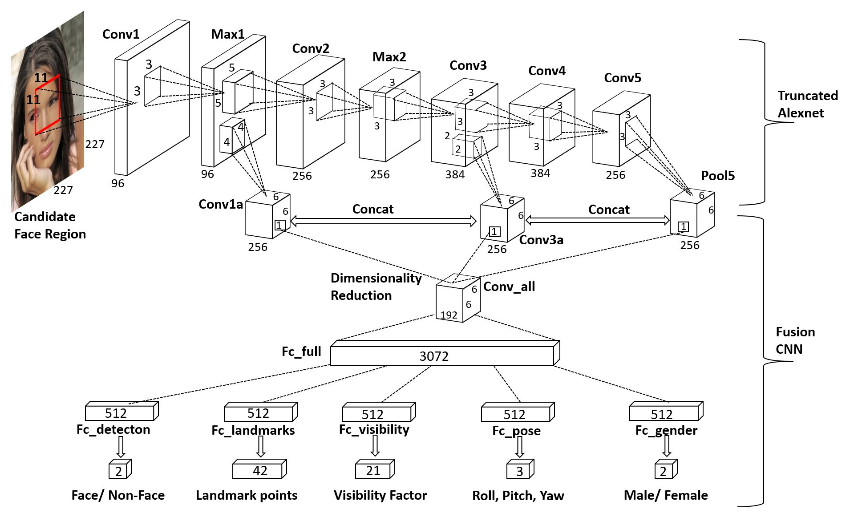
\includegraphics[scale=0.5]{fig/hyperface_structure}
\end{figure}
}

\only<2>{
\begin{figure}
\centering
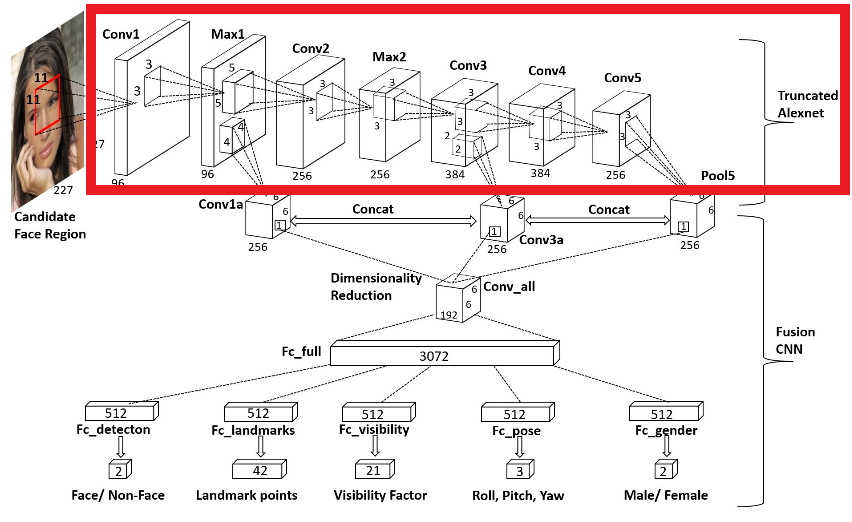
\includegraphics[scale=0.5]{fig/hyperface_structure1}
\end{figure}
}

\only<3>{
\begin{figure}
\centering
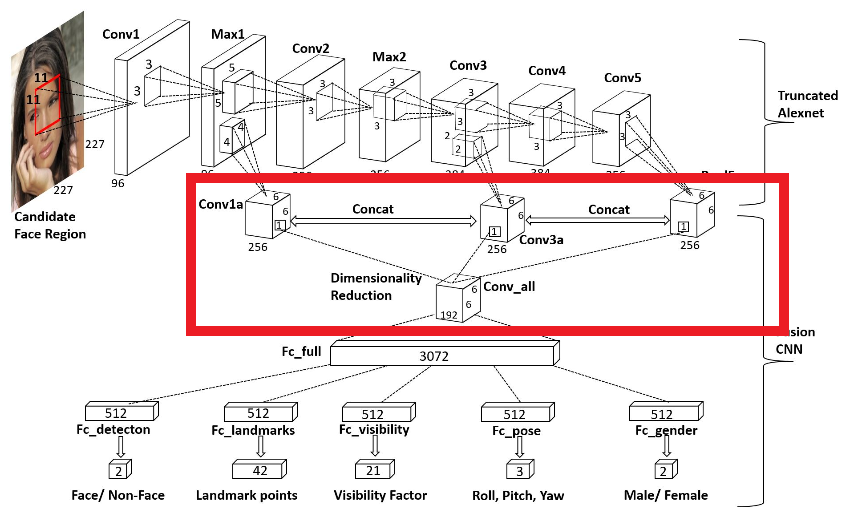
\includegraphics[scale=0.5]{fig/hyperface_structure2}
\end{figure}
}
\only<4>{
\begin{figure}
\centering
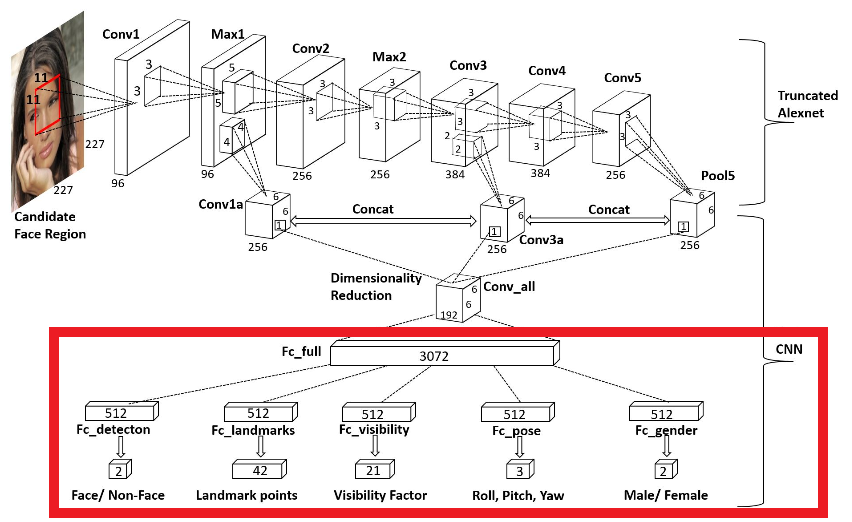
\includegraphics[scale=0.5]{fig/hyperface_structure3}
\end{figure}
}
\end{frame}


\begin{frame}{Overcoming the need for a face detector}

\onslide<1->{
1) Standard procedure: \\
Face Detector $\rightarrow$ Facebox $\rightarrow$ Predict on this box
}

\onslide<2->{
2) Hyperface: \\
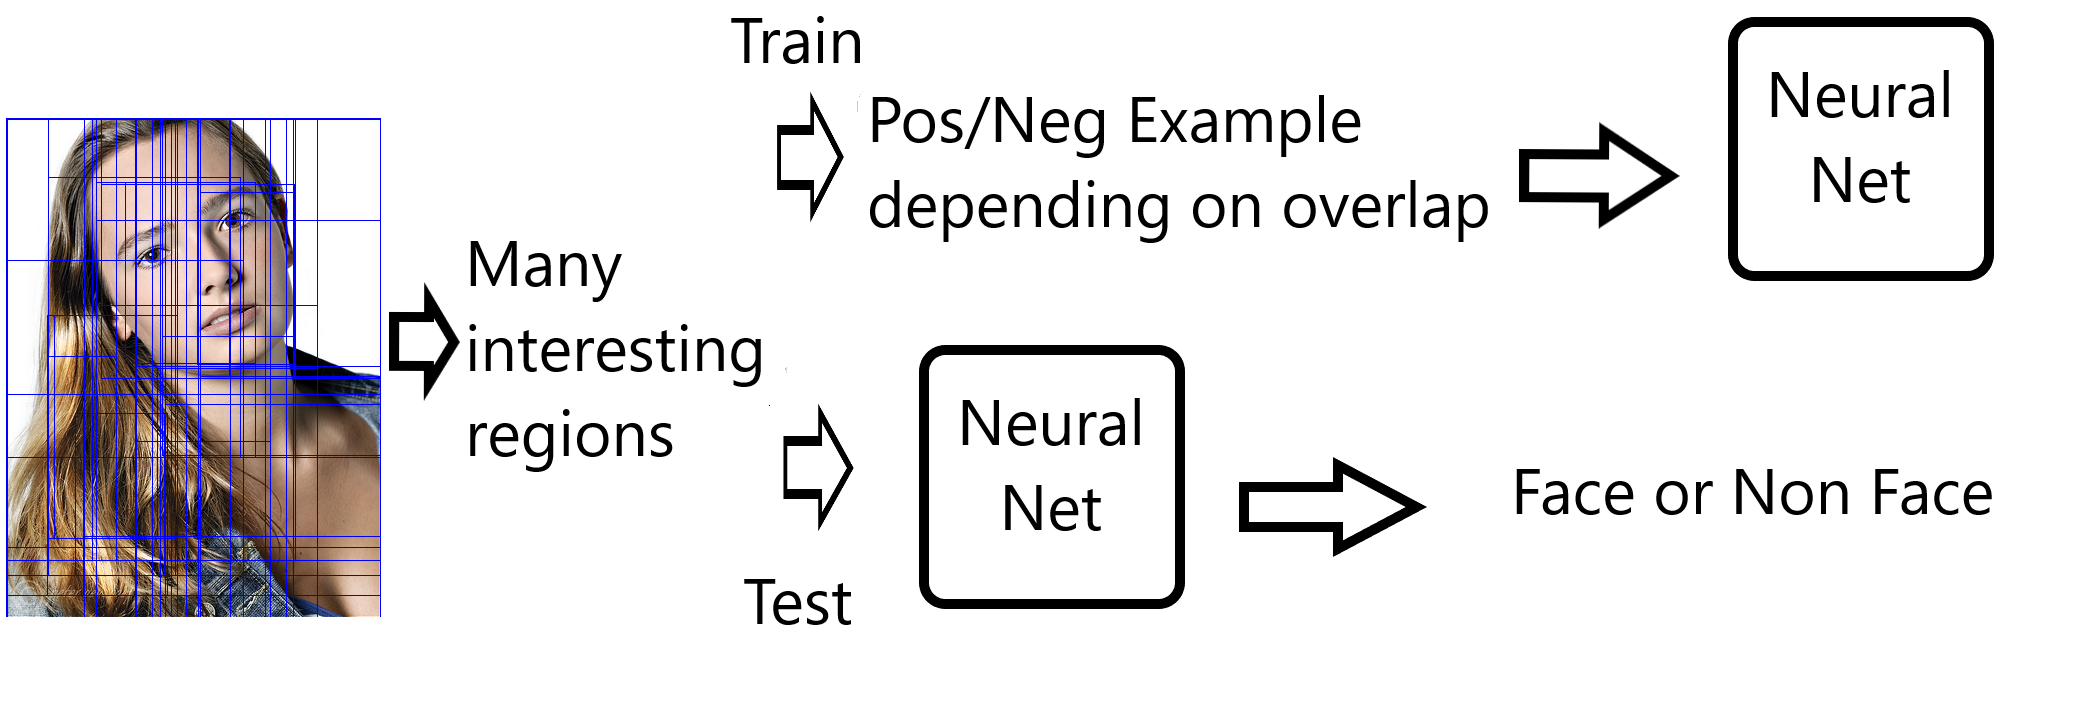
\includegraphics[scale=0.22]{fig/selective_search}
}

\end{frame}

\begin{frame}{Experiments}
\begin{center}
\begin{huge}
Experiments
\end{huge}
\end{center}
\end{frame}

\section{Experiments}
\begin{frame}{Setting}
\begin{itemize}
\item Mostly AFLW Dataset:  24'993 faces in 21'997 images
\item Use highest scoring region (face detection task)
\item Normalized Mean Error: $error = \frac{1}{N} \sum_{i = 1}^N \frac{\sqrt{(\hat{l}_i - l_i)^2}}{\sqrt{{w_f}^2 + {h_f}^2}}$
\begin{figure}
\centering
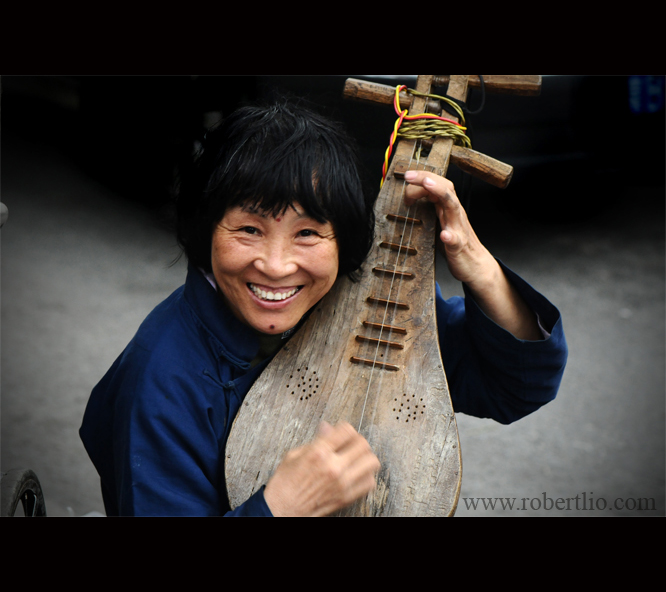
\includegraphics[scale=0.2]{fig/aflw_example2}
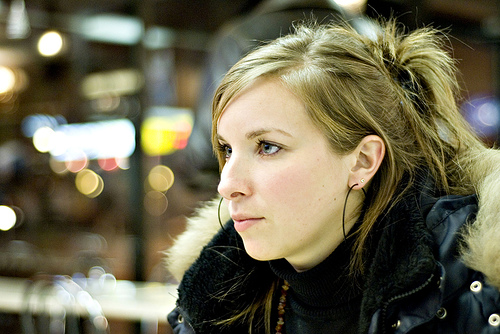
\includegraphics[scale=0.2]{fig/aflw_example3}
\end{figure}
\end{itemize}

\end{frame}


\begin{frame}{Reproducing of Paper Results}
\begin{itemize}
\item Open source framework\footnote{https://github.com/takiyu/hyperface}, not from the author of the paper\\
$\rightarrow$ Reproduce results of paper
\item Influence of pose: Split into Under \& Over
\item Over: At least one angle $>$ 45 degrees
\item Under: All angles $<$ 45 degrees
\item Discarding: Ignore image if face detection score too low
\begin{figure}
\centering
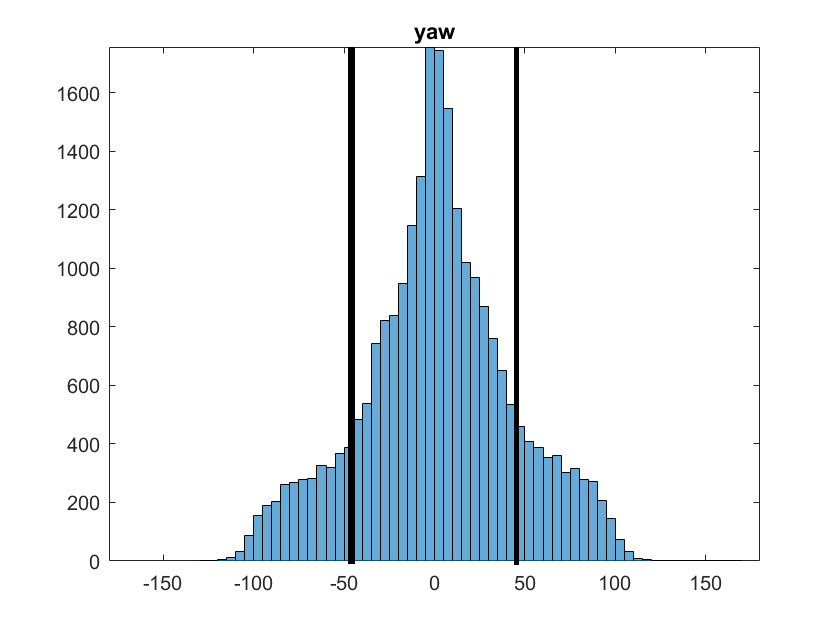
\includegraphics[scale=0.15]{fig/yaw_dist}
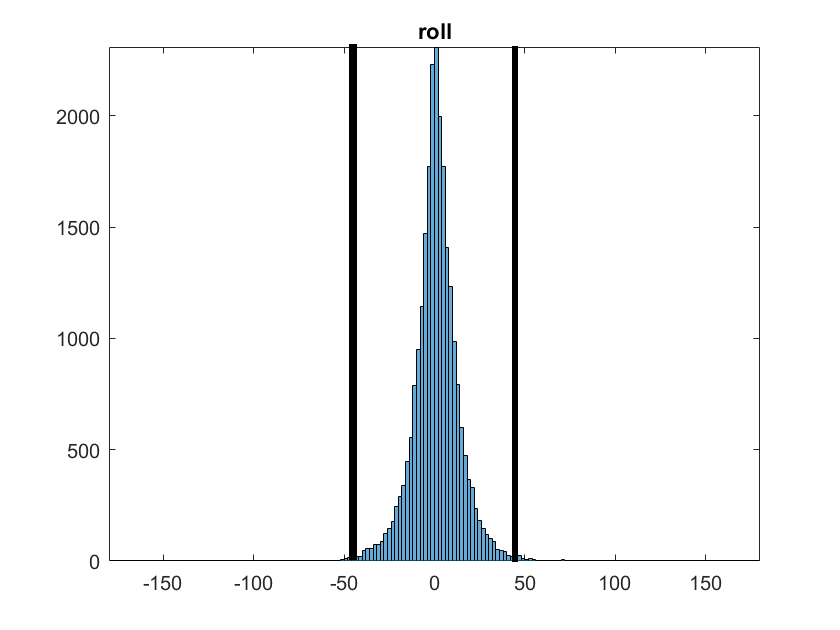
\includegraphics[scale=0.15]{fig/roll_dist}
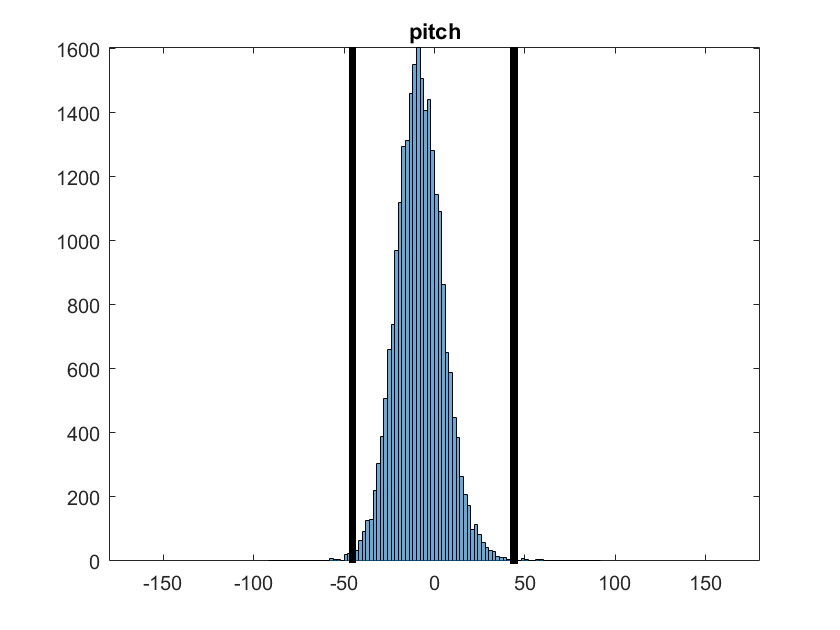
\includegraphics[scale=0.15]{fig/pitch_dist}
\end{figure}
\end{itemize}

\end{frame}

\begin{frame}{Reproducing of Paper Results - Landmarks}

\only<1>{
\begin{figure}
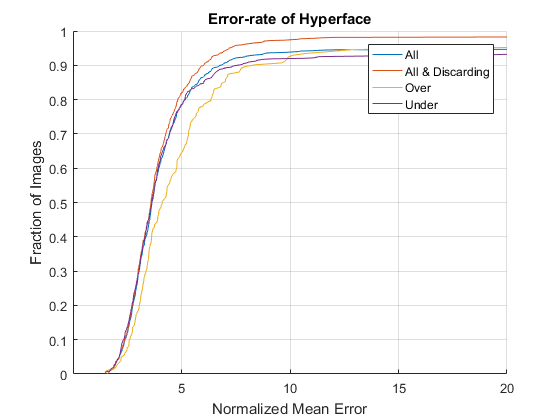
\includegraphics[scale=0.6]{fig/error_rate_eval_all_splits_and_alldisc}
\end{figure}
}
\only<2>{
\begin{figure}
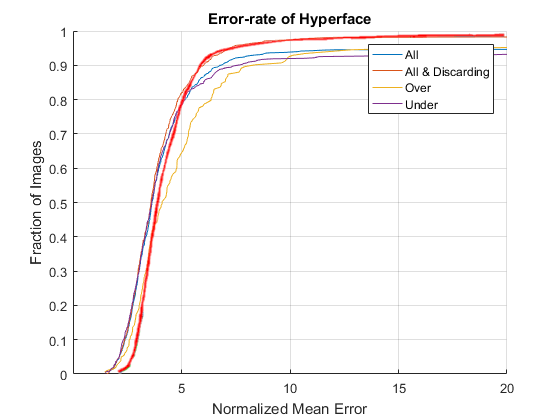
\includegraphics[scale=0.6]{fig/error_rate_eval_all_splits_and_alldisc_vs_orig_inserted}
\end{figure}
}

\end{frame}

\begin{frame}{Reproducing of Paper Results - Pose}

\begin{figure}

\subfigure[All \& Discarding]{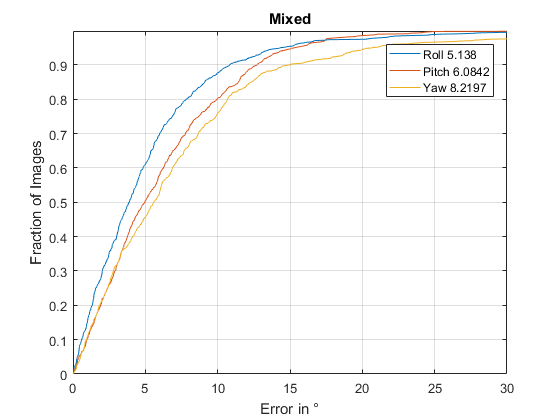
\includegraphics[scale=0.5]{fig/mixed_pose_error_all_det5}}
\end{figure}
\end{frame}

\begin{frame}{Reproducing of Paper Results - Visibility}

\begin{figure}
\centering
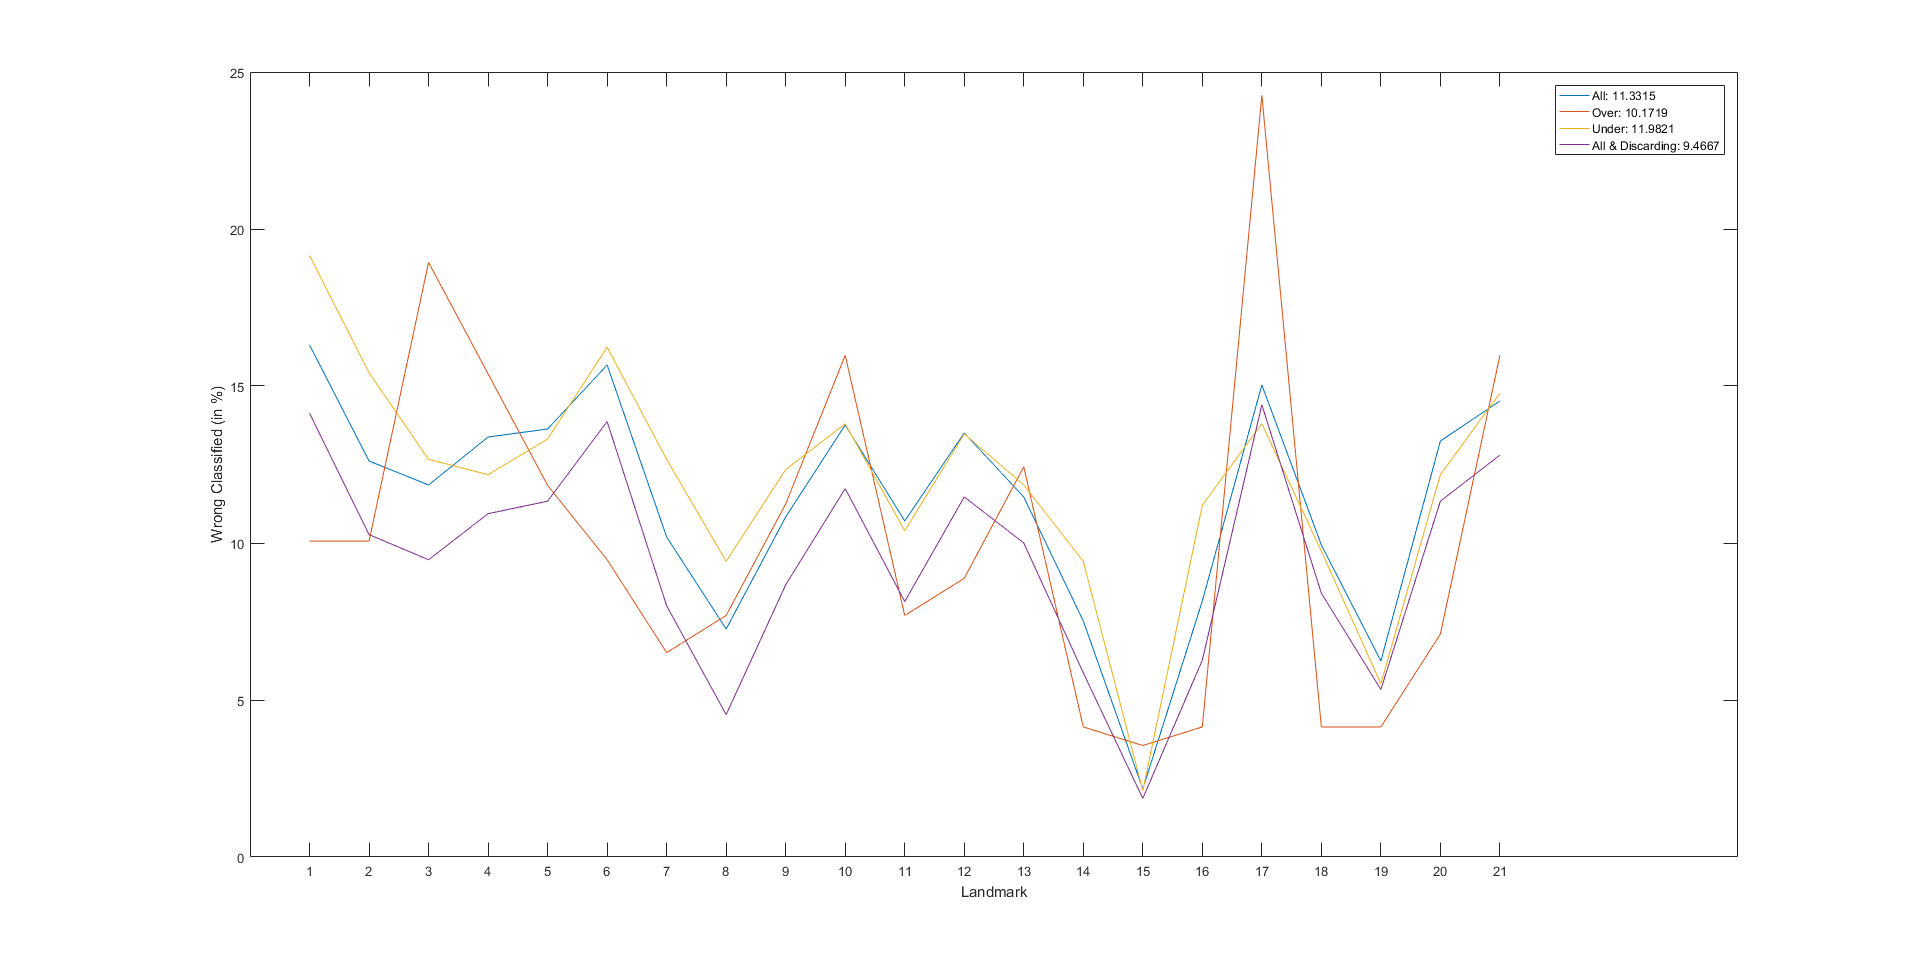
\includegraphics[scale=0.25]{fig/mixed_visibility_error_eval}
\end{figure}
\end{frame}

\begin{frame}{Problem}
\begin{figure}
\centering
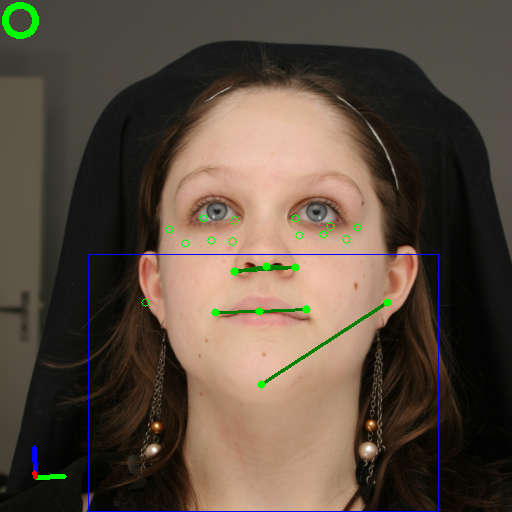
\includegraphics[scale=0.25]{fig/example_bad_box}
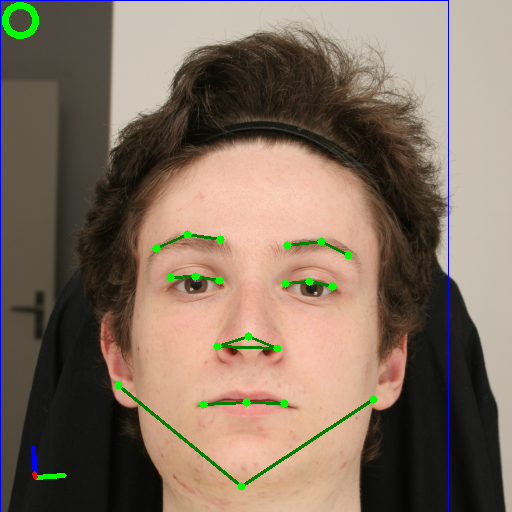
\includegraphics[scale=0.25]{fig/example_good_box}
\end{figure}
\begin{itemize}
\item Highest scoring regions sometimes not optimal
\end{itemize}
\end{frame}

\begin{frame}{Recall}
\begin{itemize}
\item Reproduction? \checkmark
\item Improve Accuracy?
\item \color{gray}{Synthetic Data in Training?} 
\end{itemize}
\end{frame}


\begin{frame}{Reminder - Selective Search}
\onslide<1->{
\begin{figure}
\centering
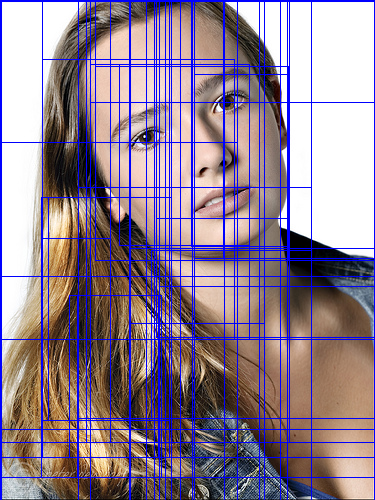
\includegraphics[scale=0.2]{fig/ss_example1}
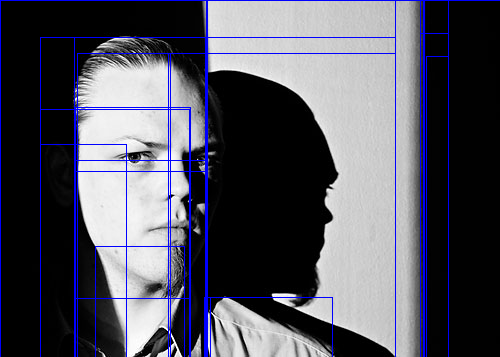
\includegraphics[scale=0.2]{fig/ss_example2}
\end{figure}

}

\onslide<2->{
\begin{itemize}
\item Idea: Average over the different regions
\end{itemize}
}
\end{frame}

\begin{frame}{Improving Accuracy - Result}

\onslide<1->{
\begin{figure}
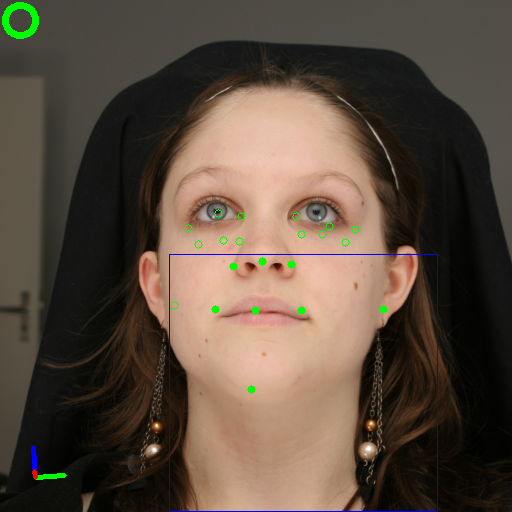
\includegraphics[scale=0.15]{fig/box_example1}
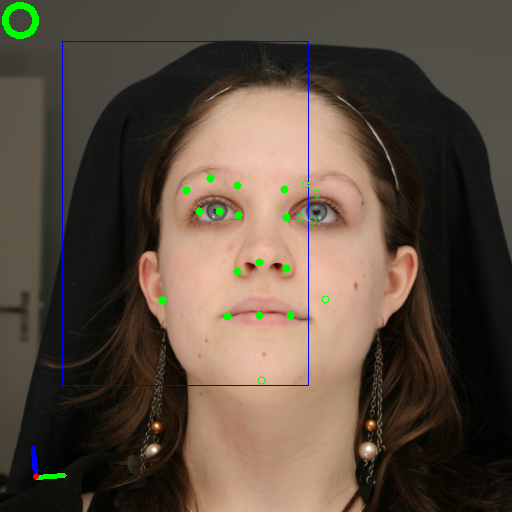
\includegraphics[scale=0.15]{fig/box_example2}
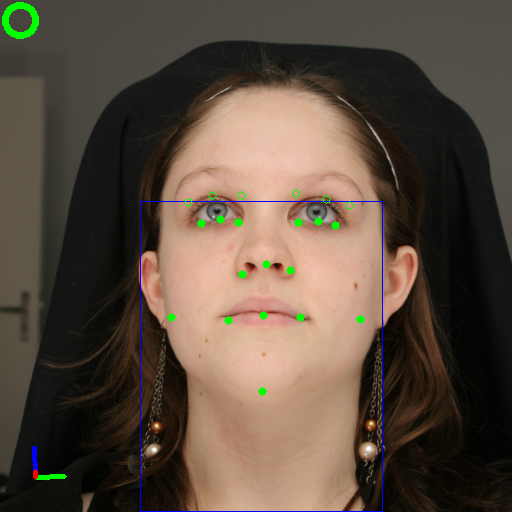
\includegraphics[scale=0.15]{fig/box_example3}
\end{figure}
}
\onslide<2>{
\begin{figure}
\centering
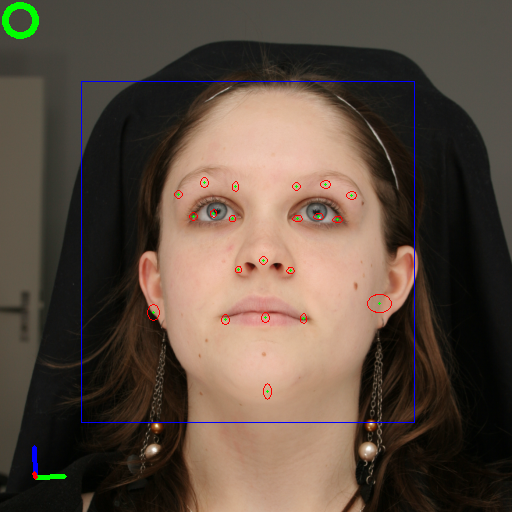
\includegraphics[scale=0.25]{fig/mean_bad_box}
\end{figure}
}
\end{frame}

\begin{frame}{Improving Accuracy - Result}

\begin{figure}
\centering
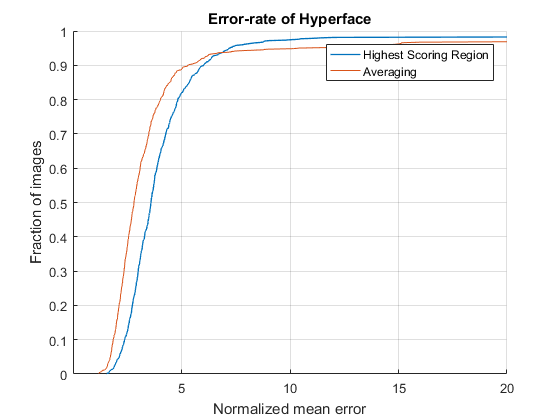
\includegraphics[scale=0.6]{fig/error_rate_mean_vs_highest}
\end{figure}
\end{frame}


\begin{frame}{Improving Accuracy - Result}

\begin{figure}
\centering
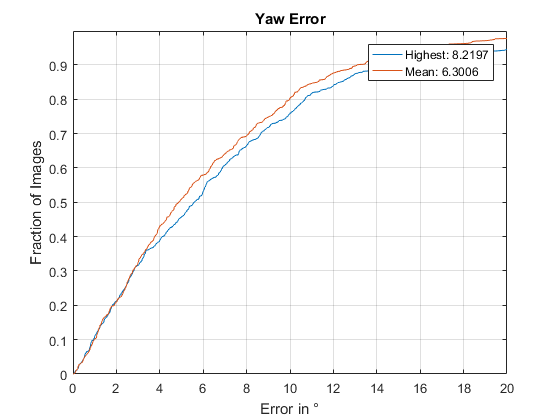
\includegraphics[scale=0.32]{fig/yaw_pose_error_mean_vs_highest}
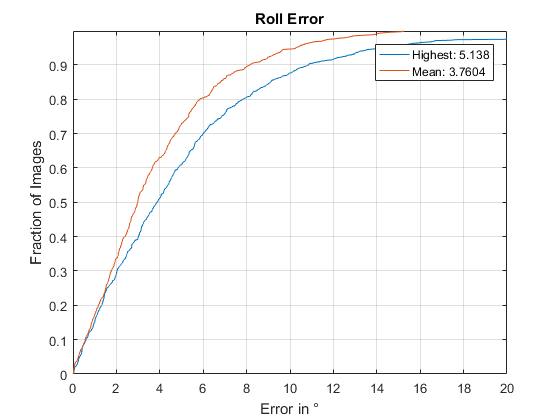
\includegraphics[scale=0.32]{fig/roll_pose_error_mean_vs_highest}
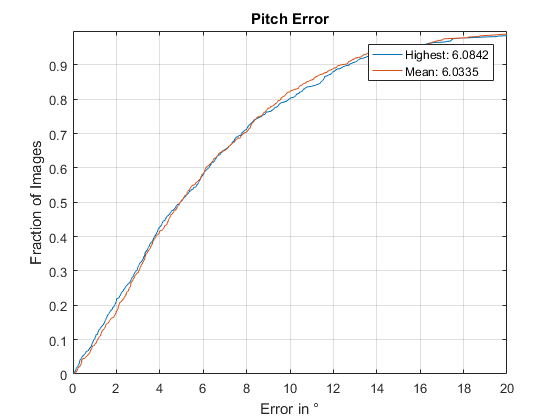
\includegraphics[scale=0.32]{fig/pitch_pose_error_mean_vs_highest}
\end{figure}
\end{frame}

\begin{frame}{Qualitative Results}
\begin{figure}
\iffalse
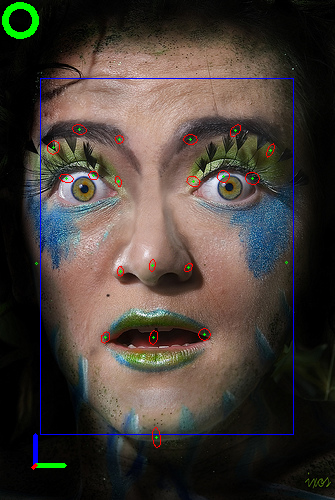
\includegraphics[scale=0.22]{fig/mean_example_pres4}
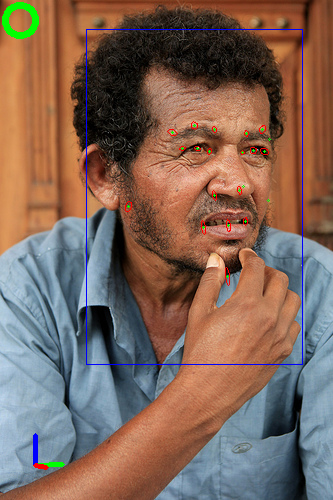
\includegraphics[scale=0.22]{fig/mean_example_pres2}
\fi
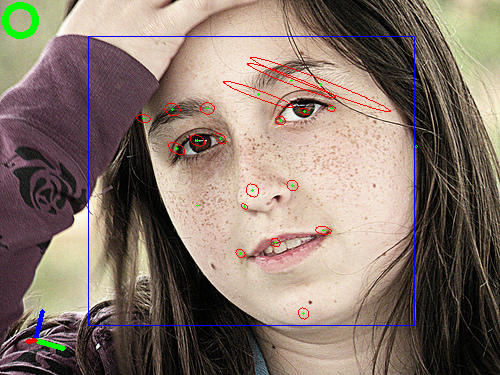
\includegraphics[scale=0.25]{fig/mean_example_pres6}
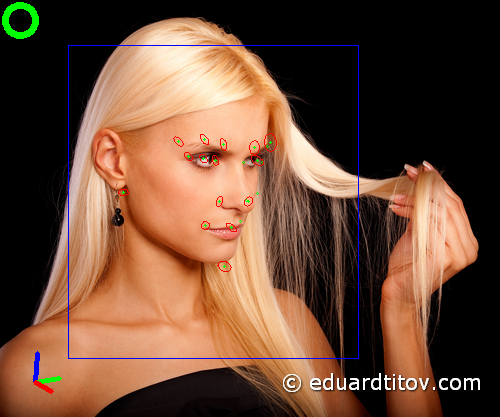
\includegraphics[scale=0.25]{fig/mean_example_pres}
\end{figure}
\end{frame}

\begin{frame}{Synthetic Training Data}
\begin{center}
\begin{huge}
Synthetic Training Data
\end{huge}
\end{center}
\end{frame}


\begin{frame}{Synthetic Training Data}

\begin{itemize}
\item High dependency on real world data
\item Synthetic data for training\footnote{https://github.com/unibas-gravis/parametric-face-image-generator}
\end{itemize}
\begin{figure}
\centering
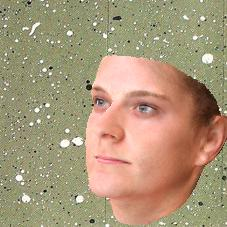
\includegraphics[scale=0.45]{fig/13_0}
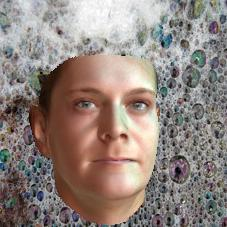
\includegraphics[scale=0.45]{fig/13_1}

\end{figure}

\end{frame}


\begin{frame}{Synthetic Training Data - Result on Synthetic Data}
\begin{figure}
\centering
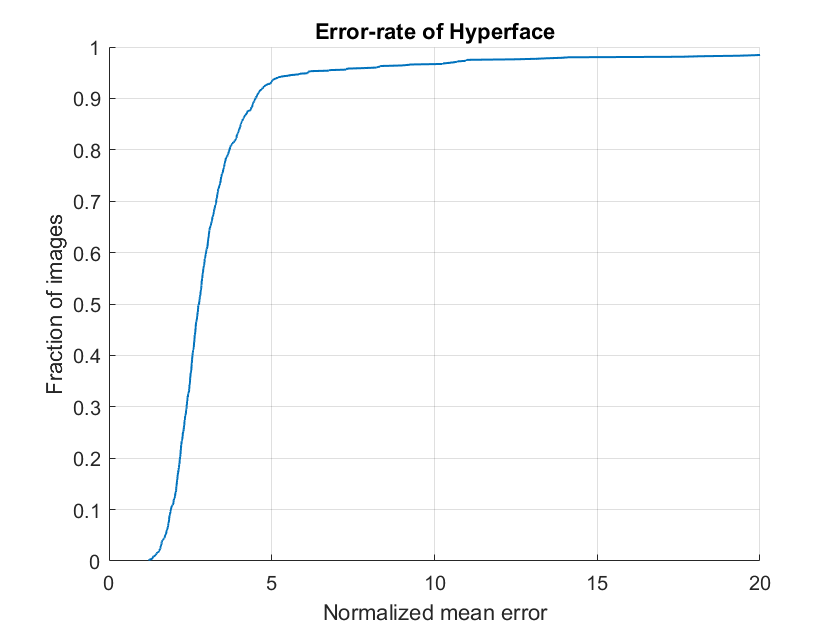
\includegraphics[scale=0.45]{fig/error_rate_synth_synth}
\end{figure}
\end{frame}

\begin{frame}{Synthetic Training Data - Result on Real World Data}
\begin{figure}
\centering
\includegraphics[scale=0.6]{fig/error_rate_synth_on_aflw}
\end{figure}
\end{frame}




\begin{frame}{Tuning with Real Word Data}

\begin{itemize}
\item Further train the network with real world data
\end{itemize}
\begin{figure}
\centering
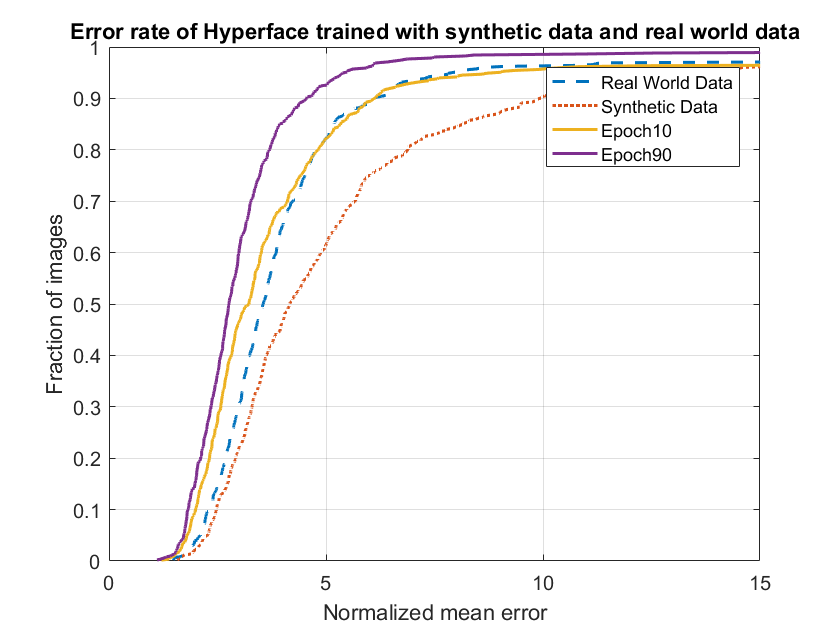
\includegraphics[scale=0.4]{fig/error_rate_synth_real2}
\end{figure}

\end{frame}

\section{Conclusion}

\begin{frame}{Conclusion}
\only<1>{
\begin{itemize}
\item Reproduction? \checkmark
\item \color{gray}{Improve Accuracy?} 
\item \color{gray}{Synthetic Data in Training?} 
\end{itemize}
}

\only<2>{
\begin{itemize}
\item Reproduction? \checkmark
\item Improve Accuracy \checkmark (+ Uncertainty) \\
$\rightarrow$ Average over regions
\item \color{gray}{Synthetic data in training?}
\end{itemize}

}

\only<3>{
\begin{itemize}
\item Reproduction? \checkmark
\item Improve Accuracy? \checkmark (+ Uncertainty)\\
$\rightarrow$ Average over regions
\item Synthetic data in training? \checkmark \\
$\rightarrow$ Tuning gives state-of-the-art-performance
\end{itemize}
}
\end{frame}

\section{Outlook}
\begin{frame}{Outlook}

\begin{itemize}

\item Leverage Uncertainty: Online Learning
\item Increase quality of synthetic data
\item Combine tuned network with averaging
\item Change thresholds
\end{itemize}
\end{frame}

\end{document}